\documentclass{beamer}
\usetheme[faculty=econ]{fibeamer}

\usepackage[utf8]{inputenc}
\usepackage[francais]{babel}
\usepackage[T1]{fontenc}
\usepackage{xcolor}

\lstset{
  language=Java,                
  basicstyle=\footnotesize,
  escapeinside={*@}{*@},
  frame=single,
  xleftmargin=2mm,
  xrightmargin=2mm,
  keepspaces=true,
  tabsize=2
}
\newcounter{ctr1}
\title[]{\Large{Développement d'applications modulaires en Java}}
\author[C. Tibermacine]{\large{Chouki~Tibermacine}\\
  \small{Chouki.Tibermacine@umontpellier.fr}}
%\institute{Polytech Montpellier}
\date{\tiny{}}

\begin{document}

\begin{frame}
\titlepage
\begin{flushright}

\includegraphics[width=3.5cm]{figs/polytech.png}
\end{flushright}
\end{frame}

\begin{frame}
  \frametitle{Références bibliographiques}
  \begin{tikzpicture}[overlay,remember picture]
    \node[anchor=center,xshift=-120pt,yshift=-20pt]
    at (current page.center) {
      
\includegraphics[width=4cm]{img/book.jpg}
    };
  \end{tikzpicture}
  \begin{tikzpicture}[overlay,remember picture]
    \node[anchor=center,xshift=60pt,yshift=-20pt]
    at (current page.center) {
      
\includegraphics[width=8cm]{img/site_web.png}
    };
  \end{tikzpicture}
  \begin{flushright}
    \vspace{4.8cm}
   {\footnotesize \url{https://maven.apache.org/guides/}}
  \end{flushright}    
\end{frame}

\AtBeginSection[]{% Print an outline at the beginning of sections
  \begin{frame}<beamer>
    \frametitle{Plan du cours}
    % \frametitle{Outline}
    \tableofcontents[currentsection]
    % \tableofcontents
  \end{frame}}

\AtBeginSubsection[]{% Print an outline at the beginning of subsections
  \begin{frame}<beamer>
    \frametitle{Plan du cours}
    % \frametitle{Outline}
    \tableofcontents[currentsubsection]
    % \tableofcontents
  \end{frame}}

\section{Introduction : besoins d'automatisation}

\begin{frame}[fragile]
  \frametitle{Au commencement, il y a avait Make}
\begin{itemize}
\item Un système de build qui s'appelle \textit{Make}
\item Très utilisé, même de nos jours, avec C sous les systèmes Unix
  notamment
\item Make permet d'écrire des \textit{Makefiles} (fichiers texte)
  avec des règles de build (compilation, clean, ...)
\item Un outil (commande \texttt{make}) interprète les règles
\item Mais problème : pas très adapté à l'éco-système Java
\end{itemize}
\end{frame}

\begin{frame}[fragile]
  \frametitle{Ensuite, il y a eu Ant}
\begin{itemize}
\item Ant pour \textit{Another Neat Tool} : un projet Apache
\item Outil Java permettant d'interpréter des règles de build
\item Les règles (\texttt{targets}) sont définies dans des fichiers
  \texttt{build.xml}
\item Avantage : flexibilité (aucune structure imposée pour le projet)
\end{itemize}
\end{frame}

\begin{frame}[fragile]
  \frametitle{Exemple avec Ant -- \texttt{build.xml}}
\begin{lstlisting}[language=Java,basicstyle=\tiny]
<project>
    <target name="clean">
        <delete dir="classes" />
    </target>
 
    <target name="compile" depends="clean">
        <mkdir dir="classes" />
        <javac srcdir="src" destdir="classes" />
    </target>
 
    <target name="jar" depends="compile">
        <mkdir dir="jar" />
        <jar destfile="jar/HelloWorld.jar" basedir="classes">
            <manifest>
                <attribute name="Main-Class"
                  value="HelloWorld" />
            </manifest>
        </jar>
    </target>
 
    <target name="run" depends="jar">
        <java jar="jar/HelloWorld.jar" fork="true" />
    </target>
</project>
\end{lstlisting}

\end{frame}

\begin{frame}[fragile]
  \frametitle{Exemple avec Ant -- A tester}
  \begin{itemize}
  \item Écrire sur un éditeur de texte une classe \texttt{HelloWorld}
    avec une méthode \texttt{main}, qui affiche le message ``Hello
    World'' et placer le fichier \texttt{HelloWorld.java} dans un
    répertoire \texttt{src}
  \item Télécharger les fichier \texttt{build.xml} depuis le dépôt Git et le
    placer à côté du répertoire \texttt{src}
  \item Taper les commandes :
\begin{enumerate}
\item \texttt{ant compile}
\item \texttt{ant jar} et ensuite \texttt{java -jar jar/HelloWorld.jar}
\item \texttt{ant run}
\end{enumerate}  
\end{itemize}

\end{frame}

\begin{frame}[fragile]
  \frametitle{Mais Ant a vite montré ses limites}
\begin{itemize}
\item Son avantage de flexibilité est devenu petit à petit son
  principal défaut :
  \begin{itemize}
  \item Des fichiers de build trop verbeux (volumineux)
  \item Trop complexes à comprendre et à maintenir
  \end{itemize}
\item Gestion des dépendances non fournie au départ :
  \begin{itemize}
  \item Pourtant très importante, surtout dans les gros projets
  \item Solution proposée : \textit{Ivy} -- un autre (sous-)projet
    d'Apache intégré à Ant
  \item Mais les développeurs Java étaient petit à petit lassés
    d'utiliser cette paire d'outils
  \end{itemize}    
\end{itemize}
\end{frame}

\begin{frame}[fragile]
  \frametitle{Et Maven est né !!!}
\begin{itemize}
\item Un système de build, mais aussi de gestion de dépendances
\item Il garde la syntaxe XML pour les fichiers de config
\item Mais contrairement à Ant, Maven privilégie \textbf{la convention
    sur la configuration} (configurations/règles implicites)
\item Ceci permet d'avoir des configurations plus concises
\item Le fichier de config s'appelle par convention \texttt{pom.xml}
  (POM pour \textit{Project Object Model})
\end{itemize}
\end{frame}

\begin{frame}[fragile]
  \frametitle{Un premier exemple avec Maven -- \texttt{pom.xml} }
  \begin{tikzpicture}[overlay,remember picture]
    \node[anchor=east,xshift=0pt,yshift=-90pt]
    at (current page.east) {
      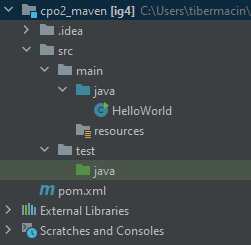
\includegraphics[width=3cm]{img/mvn_ide.png}
    };
  \end{tikzpicture}
\begin{lstlisting}[language=XML,basicstyle=\tiny]  
<?xml version="1.0" encoding="UTF-8"?>
<project xmlns="http://maven.apache.org/POM/4.0.0"
  xmlns:xsi="http://www.w3.org/2001/XMLSchema-instance"
  xsi:schemaLocation="http://maven.apache.org/POM/4.0.0 http://maven.apache.org/xsd/maven-4.0.0.xsd">
  <modelVersion>4.0.0</modelVersion>
  <groupId>ig4</groupId>
  <artifactId>HelloWorld</artifactId>
  <version>1.0-SNAPSHOT</version>
  <properties>
    <maven.compiler.source>16</maven.compiler.source>
    <maven.compiler.target>16</maven.compiler.target>
  </properties>
</project>
\end{lstlisting}
Généré automatiquement sur votre IDE :\\
\textit{Nouveau Projet Maven}\\
Sur certaines IDEs, on doit ajouter :\\
\texttt{<properties> ... </properties>}
\vspace{4.5cm}
\end{frame}

\begin{frame}[fragile]
  \frametitle{Un premier exemple avec Maven -- A tester}
\begin{itemize}
\item En ligne de commande, on peut utiliser \texttt{mvn} pour créer
  un nouveau projet avec un Archétype (\textit{template de projet}) :\\
 \texttt{mvn -B archetype:generate \ 
  -DarchetypeGroupId=org.apache.maven.archetypes \
  -DgroupId=com.mycompany.app \
  -DartifactId=my-app}
\item Penser à ajouter dans le POM l'élément properties du slide
  précédent
\end{itemize}  
\end{frame}

\begin{frame}[fragile]
  \frametitle{Le \texttt{pom.xml} obtenu {\normalsize (\url{https://maven.apache.org})}}
\begin{lstlisting}[language=XML,basicstyle=\tiny]
<project xmlns="http://maven.apache.org/POM/4.0.0"
         xmlns:xsi="http://www.w3.org/2001/XMLSchema-instance"
         xsi:schemaLocation="http://maven.apache.org/POM/4.0.0
           http://maven.apache.org/maven-v4_0_0.xsd">
  <modelVersion>4.0.0</modelVersion>
  <groupId>com.mycompany.app</groupId>
  <artifactId>my-app</artifactId>
  <packaging>jar</packaging>
  <version>1.0-SNAPSHOT</version>
  <name>my-app</name>
  <url>http://maven.apache.org</url>
  <properties>
    <maven.compiler.source>16</maven.compiler.source>
    <maven.compiler.target>16</maven.compiler.target>
  </properties>
  <dependencies>
    <dependency>
      <groupId>junit</groupId>
      <artifactId>junit</artifactId>
      <version>4.12</version>
      <scope>test</scope>
    </dependency>
  </dependencies>
</project>
\end{lstlisting}
En ligne de commande : \texttt{mvn compile}
\end{frame}

\begin{frame}[fragile]
  \frametitle{La structure obtenue {\normalsize(\url{https://maven.apache.org})}}
    \begin{tikzpicture}[overlay,remember picture]
    \node[anchor=center,xshift=0pt,yshift=20pt]
    at (current page.center) {
      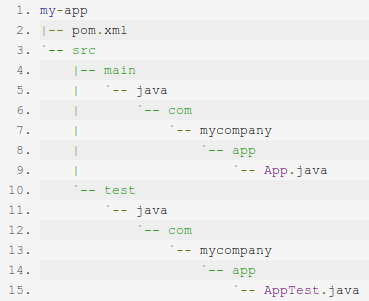
\includegraphics[width=6cm]{img/mvn_structure_rep.png}
    };
  \end{tikzpicture}  
  \begin{itemize}
    \vspace{4cm}
  \item Notez la structure (générée automatiquement) : $src/main/java$
    et $src/test/java$
  \item Structure recommandée si création de projet à la main    
  \item Après le \texttt{mvn compile}, qu'est-ce qui se passe ?

\end{itemize}  
\end{frame}

\begin{frame}[fragile]
  \frametitle{D'autres commandes à tester}
  \begin{itemize}
  \item Compiler les tests (sans les exécuter) : \texttt{mvn test-compile}
  \item Compiler et exécuter les tests : \texttt{mvn test}
  \item Créer un jar : \texttt{mvn package} (par défaut, le packaging
    est fait dans un JAR)
  \item Installer le JAR dans l'entrepôt (repository) local (par défaut,
    c'est le répertoire \texttt{\$\{user.home\}/.m2/repository}) :\\ 
    \texttt{mvn install}
  \item Effacer le répertoire \texttt{target} et partir sur une base
    propre :\\ \texttt{mvn clean}
  \item Plein d'autres commandes 
    
  \end{itemize}  
\end{frame}

\begin{frame}[fragile]
  \frametitle{Inclure des ressources dans le JAR}
  \begin{tikzpicture}[overlay,remember picture]
    \node[anchor=west,xshift=0pt,yshift=0pt]
    at (current page.west) {
      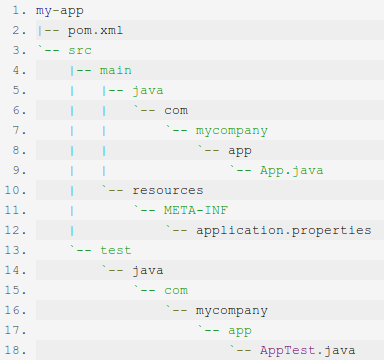
\includegraphics[width=6cm]{img/include_jar1.png}
    };
  \end{tikzpicture}
  \begin{tikzpicture}[overlay,remember picture]
    \node[anchor=east,xshift=0pt,yshift=0pt]
    at (current page.east) {
      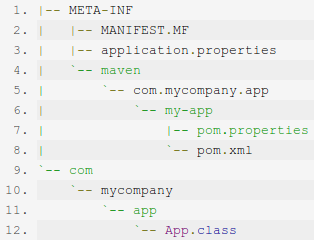
\includegraphics[width=6cm]{img/include_jar2.png}
    };
  \end{tikzpicture}
\end{frame}

\begin{frame}[fragile]
  \frametitle{Inclure des ressources pour les tests dans le JAR}
  \begin{tikzpicture}[overlay,remember picture]
    \node[anchor=west,xshift=0pt,yshift=0pt]
    at (current page.west) {
      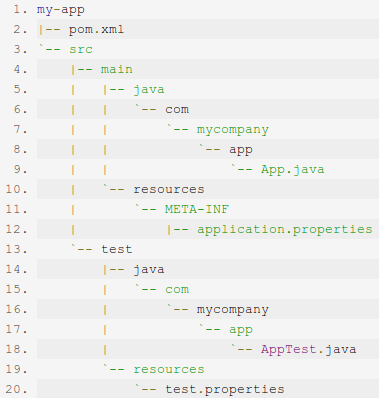
\includegraphics[width=6cm]{img/include_test_jar1.png}
    };
  \end{tikzpicture}
  \begin{tikzpicture}[overlay,remember picture]
    \node[anchor=east,xshift=0pt,yshift=0pt]
    at (current page.east) {
      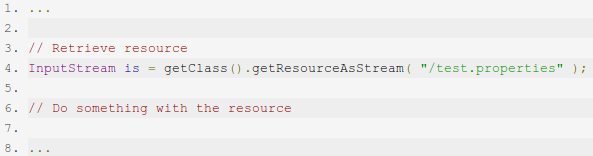
\includegraphics[width=6cm]{img/include_test_jar2.png}
    };
  \end{tikzpicture}
\end{frame}

\begin{frame}[fragile]
  \frametitle{Retour sur la structure de base d'un POM}
  \begin{itemize}
  \item \textbf{project} : élément racine
  \item \textbf{modelVersion} : version du modèle POM
  \item \textbf{groupId} : identifiant unique de l'organisation ou le
    groupe qui crée le projet (notation DNS inversée)
  \item \textbf{artifactId} : le nom unique de l'artefact généré par
    le projet (un JAR, ...). Un artefact type :
    $<artifactId>-<version>.<extension>$\\
    (ex. : $myapp-1.0.jar$)
    \item \textbf{packaging} : type de packaging (JAR, WAR, ...). JAR
      par défaut
    \item \textbf{version} : version de l'artefact généré par le
      projet
    \item \textbf{name} : nom affiché
    \item \textbf{url} : le site du projet
    \item \textbf{description}
  \end{itemize}    
\end{frame}

\begin{frame}[fragile]
  \frametitle{ça veut dire quoi \textit{SNAPSHOT} ?}
  \begin{itemize}
  \item C'est un suffixe du numéro de version
  \item Il indique que la version est en cours de développemnt
  \item Dans la version finale distribuée (la \textit{release}) le mot
    \textit{SNAPSHOT} est supprimé
  \item Ex : la version \texttt{1.0-SNAPSHOT} est distribuée comme release  \texttt{1.0}\\
    Version de développement suivante : \texttt{1.1-SNAPSHOT}
    
  \end{itemize}    
\end{frame}

\begin{frame}[fragile]
  \frametitle{Et Gradle ? le concurrent (futur substitut ?) de Maven}
\begin{itemize}
\item Un autre système de build et de gestion de dépendances
\item Objectif : Rendre le système flexible comme Ant, mais tout en
  ayant des fichiers de config petits comme dans Maven (\textit{Convention
  over Configuration})
\item Plus de XML, mais un DSL (langage dédié) inspiré de la syntaxe
  Groovy ou Kotlin
\item Multi-langages : Java, Scala, ...
\item Les étapes de build s'appellent des tâches (\textit{tasks})
\item Un système minimaliste couplé à un gros éco-système de plugins
\end{itemize}
\end{frame}

\begin{frame}[fragile]
  \frametitle{Exemple avec Gradle -- Fichier de config. \texttt{build.gradle}}
\begin{lstlisting}[basicstyle=\scriptsize]
apply plugin: 'java'
 
repositories {
    mavenCentral()
}
 
jar {
    baseName = 'gradleExample'
    version = '0.0.1-SNAPSHOT'
}
 
dependencies {
    compile 'junit:junit:4.12'
}
\end{lstlisting}
Plugin \texttt{java} pour pouvoir compiler (commande : \texttt{gradle
  classes})
\end{frame}

\section{Cycle de vie, phases et goals}
\begin{frame}[fragile]
  \frametitle{Cycle de vie d'un build}
\begin{itemize}
\item Le processus de build et de distribution d'artefacts (un JAR par
  exemple) est explicitement défini par son ``cycle de vie''
\item Pour un développeur, il suffit de taper de simples commandes et
  dans le POM il y a tout le nécessaire pour obtenir les résultats voulus
\item Trois types de cycles de vie :
  \begin{itemize}
  \item \texttt{default} ou \texttt{build} : gère le déploiement du
    projet
  \item \texttt{clean} : gère le nettoyage du projet
  \item \texttt{site} : gère la création du site de documentation du projet
  \end{itemize}
\item Chaque cycle de vie est constitué d'une liste de \textit{phases}
\end{itemize}
\end{frame}

\begin{frame}[fragile]
  \frametitle{Phases d'un cycle de vie}
\begin{itemize}
\item  Pour le cycle de vie par défaut (\textbf{\texttt{default}} ou \textbf{\texttt{build}})
  \begin{enumerate}
  \item \textbf{\texttt{validate}} : valider que le projet est correct et que
    toute l'information nécessaire est disponible
  \item \textbf{\texttt{compile}} : compiler le code source du projet
  \item \textbf{\texttt{test}} : tester le code compilé en utilisant un
    framework de tests unitaires (jUnit par ex.)
  \item \textbf{\texttt{package}} : empaqueter le code compilé dans un format
    ``distribuable'', un JAR par ex.
  \item \textbf{\texttt{verify}} : exécuter n'importe quelles vérifications sur
    les résultats des tests d'intégration
  \item \textbf{\texttt{install}} : installer le paquet dans un \textit{repo.}
    local pour être utilisé comme dépendance dans d'autres projets
    locaux
  \item \textbf{\texttt{deploy}} : fait dans l'environnement de build en
    copiant le package final dans un repo distant pour partager le
    projet avec d'autres développeurs/projets
  \end{enumerate}
\end{itemize}
\end{frame}

\begin{frame}[fragile]
  \frametitle{Exécuter une phase via une commande}
\begin{itemize}
\item Le fait d'exécuter une commande avec une phase va provoquer
  l'exécution de toutes les phases en amont dans le cycle de vie
\item Exemple :
  \begin{itemize}
  \item exécuter ``\texttt{mvn install}''
  \item provoque l'exécution de toutes les phases du cycle de vie par
    défaut, jusqu'à la phase \texttt{install} :\\ \texttt{validate} $>$
    \texttt{compile} $>$ \texttt{test} $>$ \texttt{package} $>$ \texttt{verify}
    $>$ \texttt{install}
  \end{itemize}
\item On peut exécuter des commandes relevant de différents cycles de vie :
  \begin{itemize}
  \item Exemple : ``\texttt{mvn clean deploy}''
  \item nettoie (cycle de vie \texttt{clean}) et ensuite déploie
  \end{itemize}
\end{itemize}
\end{frame}

\begin{frame}[fragile]
  \frametitle{Objectifs (\textit{Goals}) des plugins}
\begin{itemize}
\item En réalité, une phase est constituée d'``\textit{objectifs}''
  contribués par des plugins
\item Exemple :\\ \texttt{mvn clean dependency:copy-dependencies package}
  \begin{itemize}
  \item \texttt{clean} et \texttt{package} sont des phases auxquelles
    sont associées des objectifs implicites par défaut
    (\texttt{clean:clean} et \texttt{jar:jar})
  \item \texttt{copy-dependencies} est un objectif d'un plugin
    \texttt{dependency}
  \item les objectifs sont exécutés dans l'ordre
\end{itemize}
% \item Un objectif peut être lié à une ou plusieurs phases (il est
%   exécuté dans chaque phase) et inversement (tous les objectifs seront
%   exécutés lors de l'exécution de la phase)
\end{itemize}
\end{frame}

\begin{frame}[fragile]
  \frametitle{Personnaliser le cycle de vie d'un projet}
Deux façons de faire :   
  \begin{itemize}    
  \item personnaliser le packaging
    \begin{itemize}    
    \item Élément POM packaging à éditer (packaging JAR par défaut)
    \item Pour le packaging JAR :\\
      \begin{tabular}{|l|l|}        
        \hline
        \textbf{phase} & \textbf{plugin:goal}  \\
        \hline
        ... & ...\\
        \hline
        \texttt{compile} & \texttt{compiler:compile} \\
        \hline
        \texttt{test} & \texttt{surefire:test} \\
        \hline
        \texttt{package} & \texttt{jar:jar} \\
        \hline
        ... & ...\\
        \hline
\end{tabular}

    \end{itemize}
  \item ajouter des objectifs en configurant des plugins
    \begin{itemize}    
    \item Un plugin : un artefact contribuant avec des objectifs
    \item Exemple : Plugin \textit{Compiler} contribue avec deux
      objectifs \texttt{compile} pour compiler le code source du
      projet et \texttt{testCompile} pour compiler les classes de test
    \end{itemize}
\end{itemize}
\end{frame}

\begin{frame}[fragile]
  \frametitle{Personnaliser le cycle de vie d'un projet -suite-}
  \begin{block}{Configurer un plugin}
    \begin{enumerate}
    \item Ajouter un élément \texttt{plugin} dans le POM (sous
      l'élément \texttt{plugins})
    \item Indiquer les objectifs/\textit{goals} (l'intégration seule
      du plugin ne suffit pas)
    \end{enumerate}
  \end{block}
  \begin{itemize}
  \item Ces objectifs vont s'ajouter aux objectifs déjà affectés à la
    phase du cyle de vie (indiquée dans le POM sous l'élément
    \texttt{plugin})
  \item Ils vont s'exécuter après ceux déjà affectés à la phase
  \item Il est possible de changer l'ordre (élément
    \texttt{executions})
  \end{itemize}
\end{frame}

\begin{frame}[fragile]
	\frametitle{Personnaliser le cycle de vie d'un projet -suite-}
	Ex : rendre le JAR produit par la phase \texttt{package} exécutable. Après l'élément \texttt{<dependencies>}, ajouter~:
\begin{lstlisting}[language=XML,basicstyle=\scriptsize]		
...
<build>
 <plugins>
  <plugin>
   <groupId>org.apache.maven.plugins</groupId>
   <artifactId>maven-jar-plugin</artifactId>
   <configuration>
    <archive>
     <manifest>
      <mainClass>HelloWorld</mainClass>
     </manifest>
    </archive>
   </configuration>
  </plugin>
 </plugins>
</build>
\end{lstlisting}
\end{frame}

\begin{frame}[fragile]
  \frametitle{Liste de plugins {\normalsize (\url{https://maven.apache.org/plugins/})}}
  \begin{tikzpicture}[overlay,remember picture]
    \node[anchor=center,xshift=0pt,yshift=-10pt]
    at (current page.center) {
      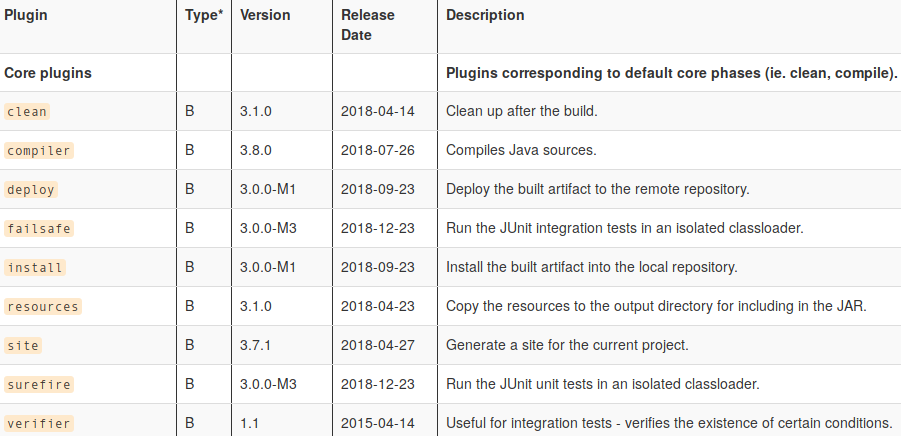
\includegraphics[width=12cm]{img/plugin_list1.png}
    };
  \end{tikzpicture}
  \begin{flushleft}
    \vspace{6cm}    
{\footnotesize    $^*$ B pour Build Plugin ou R pour Reporting plugin}
  \end{flushleft}
\end{frame}

\begin{frame}[fragile]
  \frametitle{Liste de plugins {\normalsize (\url{https://maven.apache.org/plugins/})}}
  \begin{tikzpicture}[overlay,remember picture]
    \node[anchor=center,xshift=0pt,yshift=-20pt]
    at (current page.center) {
      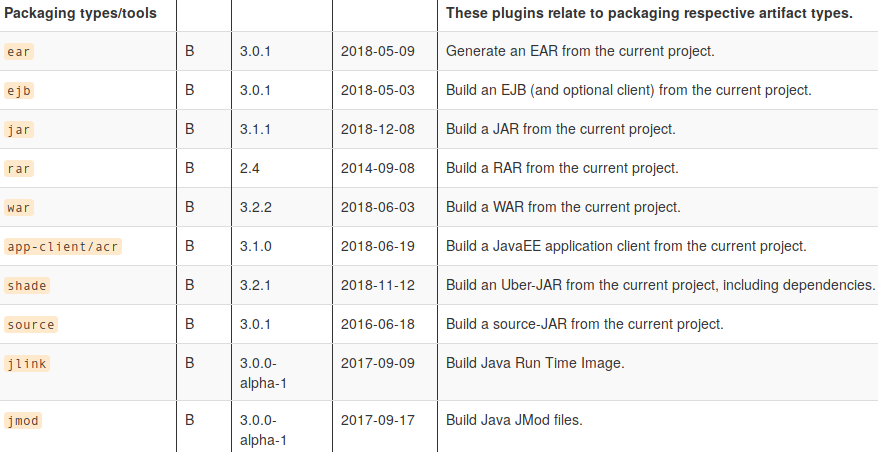
\includegraphics[width=12cm]{img/plugin_list2.png}
    };
  \end{tikzpicture}
\end{frame}

\begin{frame}[fragile]
  \frametitle{Liste de plugins {\normalsize (\url{https://maven.apache.org/plugins/})}}
  \begin{tikzpicture}[overlay,remember picture]
    \node[anchor=center,xshift=0pt,yshift=-20pt]
    at (current page.center) {
      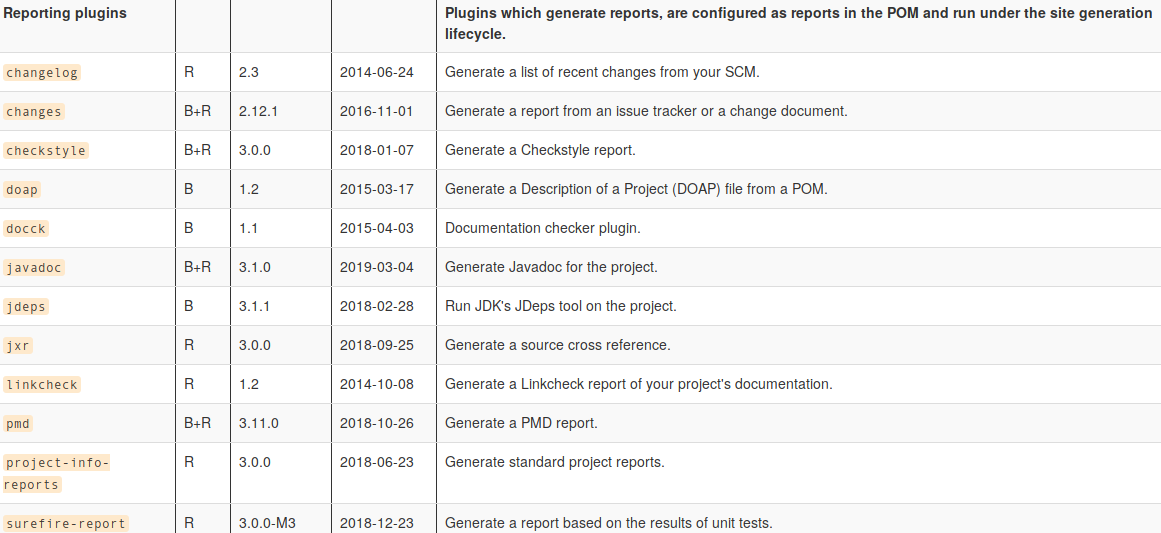
\includegraphics[width=12cm]{img/plugin_list3.png}
    };
  \end{tikzpicture}
\end{frame}

\begin{frame}[fragile]
  \frametitle{Liste de plugins {\normalsize (\url{https://maven.apache.org/plugins/})}}
  \begin{tikzpicture}[overlay,remember picture]
    \node[anchor=center,xshift=0pt,yshift=-20pt]
    at (current page.center) {
      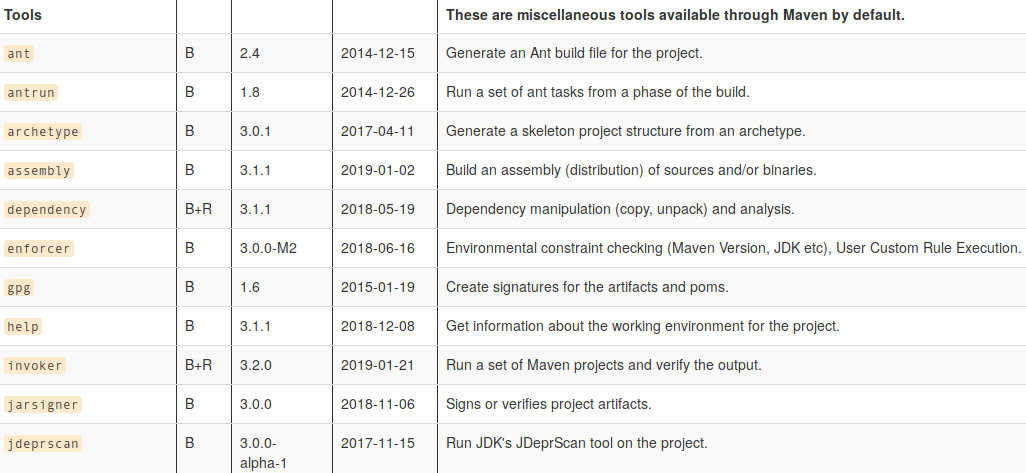
\includegraphics[width=12cm]{img/plugin_list4.png}
    };
  \end{tikzpicture}
\end{frame}

\begin{frame}[fragile]
  \frametitle{Liste de plugins {\normalsize (\url{https://maven.apache.org/plugins/})}}
  \begin{tikzpicture}[overlay,remember picture]
    \node[anchor=center,xshift=0pt,yshift=-20pt]
    at (current page.center) {
      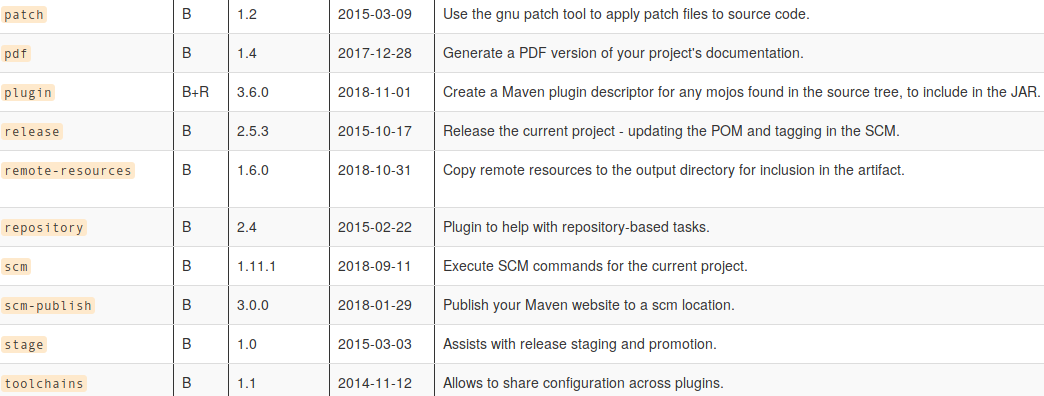
\includegraphics[width=12cm]{img/plugin_list5.png}
    };
  \end{tikzpicture}
\end{frame}

\section{Gestion des dépendances}
\begin{frame}[fragile]
  \frametitle{L'élément \texttt{dependencies/dependency} dans le POM}
\begin{itemize}
\item Dans un exemple donné avant, il y avait une dépendance déclarée
  vers jUnit dans le POM :
  \begin{lstlisting}[language=XML,basicstyle=\scriptsize]
  <dependencies>
    <dependency>
      <groupId>junit</groupId>
      <artifactId>junit</artifactId>
      <version>4.12</version>
      <scope>test</scope>
    </dependency>
  </dependencies>
\end{lstlisting}
Cette dépendance externe est nécessaire pour le build du projet lors
de la compilation, lors des tests ou à l'exécution (scope :
\textit{compile}, \textit{test} ou \textit{runtime})
\end{itemize}
\end{frame}

\begin{frame}[fragile]
  \frametitle{Où chercher les dépendances ?}
\begin{itemize}
\item Au moment du build, Maven lit les dépendances dans le POM (il y
  en a qui sont héritées du ``\textit{Super POM}'')
\item Pour chaque dépendance, il va chercher la dépendance d'abord
  dans le repo local (par défaut,
 {\footnotesize \texttt{\$\{user.home\}/.m2/repository}})
\item Sinon, il la cherche (la télécharge et l'installe dans le repo
  local) depuis des repos distants
\item Par défaut, le repo distant est \textit{Maven Central} :\\
  {\footnotesize \url{https://repo.maven.apache.org/maven2/}}\\
  Certaines entreprises ont leur propre repo
\item C'est quoi un repo. (entrepôt) : un endroit où sont stockés les
  artifacts (JAR entre autres) partagés par les projets Maven
\end{itemize}
\end{frame}

\begin{frame}[fragile]
  \frametitle{Ajouter une dépendance}
  \begin{itemize}
  \item On doit d'abord chercher les :
    \textit{groupId}, \textit{artifactId} et \textit{version}
  \item Exemple : on veut produire des logs dans notre code et on va
    utiliser log4j pour ça
  \item En parcourant le repo Maven Central, on retrouve la
    description suivante (dans le fichier \texttt{maven\_metadata.xml} de
    log4j)~:
\begin{lstlisting}[language=XML,basicstyle=\tiny]
<metadata modelVersion="1.1.0">
  <groupId>log4j</groupId>
  <artifactId>log4j</artifactId>
  <versioning>
    <latest>1.2.17</latest>
    <release>1.2.17</release>
    <versions>
      <version>1.1.3</version>
      <version>1.2.4</version>
      ...
      <version>1.2.17</version>
    </versions>
    <lastUpdated>20140318154402</lastUpdated>
  </versioning>
</metadata>
\end{lstlisting}
\end{itemize}
\end{frame}

\begin{frame}[fragile]
  \frametitle{Ajouter une dépendance -suite-}
  \begin{itemize}
  \item On va ajouter ça au POM de notre projet :
\begin{lstlisting}[language=XML,basicstyle=\scriptsize]
...
    <dependency>
      <groupId>log4j</groupId>
      <artifactId>log4j</artifactId>
      <version>1.2.17</version>
      <scope>compile</scope>
    </dependency>  
...
\end{lstlisting}
\item En faisant ensuite \texttt{mvn compile}, Maven va télécharger la
  dépendance pour nous et la mettre à disposition du compilateur (configure le CLASSPATH)
\end{itemize}
\end{frame}

\begin{frame}[fragile]
  \frametitle{Déployer des artefacts dans un repo distant}
  \begin{tikzpicture}[overlay,remember picture]
    \node[anchor=south,xshift=-35pt,yshift=0pt]
    at (current page.south) {
      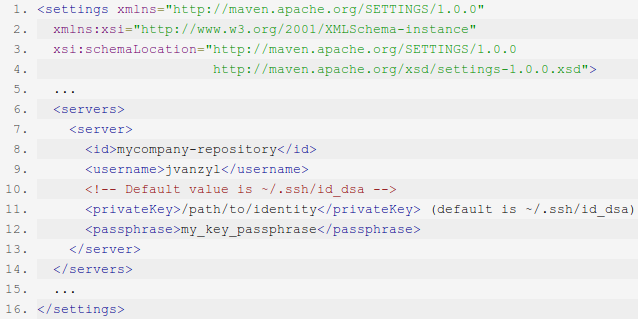
\includegraphics[width=6.5cm]{img/deploy_remote_repo.png}
    };
  \end{tikzpicture}  
  
  \begin{itemize}
  \item Il faudrait indiquer l'URL du repo dans le POM et indiquer un
    moyen d'authentifcation (settings.xml)
  \item Exemple avec scp :
\begin{lstlisting}[language=XML,basicstyle=\tiny]  
  <distributionManagement>
    <repository>
      <id>mycompany-repository</id>
      <name>MyCompany Repository</name>
      <url>scp://repository.mycompany.com/repository/maven2</url>
    </repository>
  </distributionManagement>
\end{lstlisting}    
\vspace{4cm}
  \end{itemize}
\end{frame}

\begin{frame}[fragile]
  \frametitle{Utiliser un repo interne}
  \begin{tikzpicture}[overlay,remember picture]
    \node[anchor=south,xshift=70pt,yshift=0pt]
    at (current page.south) {
      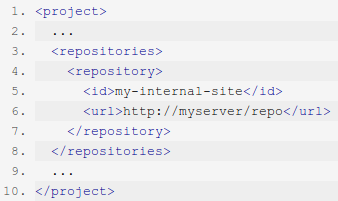
\includegraphics[width=4.5cm]{img/internal_repo.png}
    };
  \end{tikzpicture}    
  \begin{itemize}
  \item Dans certaines entreprises on utilise un repo interne pour
    déployer des projets privés 
    
  \item Il suffit d'installer un serveur de fichier ou Web organisé
    comme Maven Central ({\footnotesize
      \url{http://repo.maven.apache.org/maven2/}})
  \item Ne pas scraper ou faire un rsync de Maven Central, sous peine
    d'être bloqué
    \item Plus d'explications/outils pour gérer un repo interne :\\ {\footnotesize\url{https://maven.apache.org/repository-management.html}}
      \vspace{1cm}
    \item Pour utiliser un repo interne :
      \vspace{2cm}      
  \end{itemize}
\end{frame}

\begin{frame}[fragile]
  \frametitle{Dépendances transitives}
  \begin{itemize}
  \item Maven évite aux développeurs d'analyser et spécifier les
    dépendances requises par les dépendances d'un projet
  \item Il garantit de façon automatique des dépendances transitives
  \item Cette résolution des dépendances peut s'étendre assez
    largement (graphe de dép. peut être très large et profond)
  \item On peut avoir des problèmes d'ambiguité ou bien des problèmes
    avec des dépendances cycliques
  \item Ambiguité : Si dans le graphe de dépendances, on a :\\
    A $\rightarrow$ B $\rightarrow$ C $\rightarrow$ D[2.0]\\
    A $\rightarrow$ E $\rightarrow$ D[1.0]\\
    Maven prend D[1.0] (chemin le plus court) sinon il faut mettre la
    dépendance vers D[2.0] dans A
  \end{itemize}
\end{frame}

\begin{frame}[fragile]
  \frametitle{Exclure des dépendances}
  \begin{itemize}
  \item Il est possible dans un projet d'exclure une dépendance
    transitive
  \item Ex : X $\rightarrow$ Y $\rightarrow$ Z\\
    Dans X on peut déclarer (dans un élément \texttt{exclusion} du
    POM) qu'on exclut Z
  \item Un autre moyen d'exclure des dépendances est de les déclarer
    optionnelles (élément \texttt{optional} du POM)
  \item Ex : Y $\rightarrow$ Z\\
    Dans Y, on peut déclarer Z comme dépendance optionnelle\\
    Si X $\rightarrow$ Y, il ne sera pas dépendant de Z\\
  \end{itemize}
\end{frame}

\begin{frame}[fragile]
  \frametitle{Expliciter les dépendances tout de même}
  \begin{itemize}
  \item Supposons X $\rightarrow$ Y $\rightarrow$ Z
  \item X peut tout à fait utiliser le code dans Z
  \item Mais il est recommandé de l'expliciter dans les dépendances de
    X pour ne pas avoir des problèmes de build et pour améliorer la
    documentation de X
  \item Maven fournit un plugin \texttt{dependency} qui fournit un
    objectif \texttt{dependency:analyze} qui permet de vérifier les
    dépendances lors du build
  \end{itemize}
\end{frame}

\begin{frame}[fragile]
  \frametitle{Portée (\textit{scope}) des dépendances}
  \begin{itemize}
  \item \textbf{compile} (par défaut) : dépendances disponibles dans
    tous les classpaths du projet et sont propagées aux projets
    dépendants
  \item \textbf{provided} : ressemble beaucoup à \textit{compile},
    mais n'est pas transitive
  \item \textbf{runtime} : dépendances non requises pour la compilation
  \item \textbf{test} : dépendances requises pour la compilation et
    l'exécution des tests. N'est pas transitive
  \item \textbf{system} : comme \textit{provided}, mais le JAR de
    l'artifact requis doit être fourni (n'est pas recherché dans un
    repo)
  \item \textbf{import} : dépendance doit être remplacée par ce qui
    est indiqué dans la section \texttt{<dependencyManagement>} d'un
    POM.
  \end{itemize}
\end{frame}

\begin{frame}[fragile]
  \frametitle{Dépendance entre modules dans un projet Maven}
  \begin{tikzpicture}[overlay,remember picture]
    \node[anchor=west,xshift=0pt,yshift=0pt]
    at (current page.west) {
      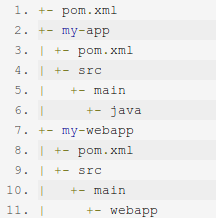
\includegraphics[width=4.5cm]{img/multi_mod_project.png}
    };
  \end{tikzpicture}
  \begin{tikzpicture}[overlay,remember picture]
    \node[anchor=east,xshift=0pt,yshift=0pt]
    at (current page.east) {
      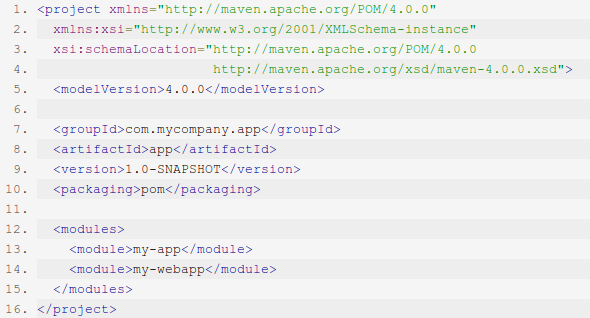
\includegraphics[width=8cm]{img/multi_mod_project2.png}
    };
  \end{tikzpicture}
\end{frame}

\begin{frame}[fragile]
  \frametitle{Dépendance entre modules dans un projet Maven}
  \begin{tikzpicture}[overlay,remember picture]
    \node[anchor=center,xshift=80pt,yshift=30pt]
    at (current page.center) {
      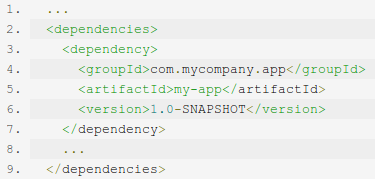
\includegraphics[width=6cm]{img/pom_multi_mod.png}
    };
  \end{tikzpicture}
  \begin{tikzpicture}[overlay,remember picture]
    \node[anchor=south,xshift=0pt,yshift=0pt]
    at (current page.south) {
      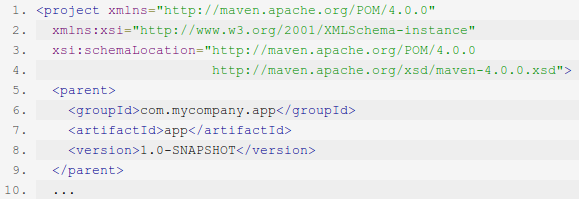
\includegraphics[width=10cm]{img/pom_multi_mod2.png}
    };
  \end{tikzpicture}
  \begin{flushleft}
    Dans \texttt{my-webapp/pom.xml}    \\
    \vspace{1.5cm}
    Ajouter \texttt{parent} dans le POM de chaque module
    \vspace{2.5cm}
  \end{flushleft}
\end{frame}

\begin{frame}
  \begin{tikzpicture}[overlay,remember picture]
    \node[anchor=center,xshift=0pt,yshift=0pt]
    at (current page.center) {
      
\includegraphics[width=4cm]{img/question.jpg}
    };
  \end{tikzpicture}
\end{frame}

\end{document}
